\chapter{Gestion automatisée du stationnement: État de l'art}
\markboth{Gestion automatisée du stationnement: État de l'art}{}

\section{Introduction}
\subsection{ Détection de visage et  localisation des points caractéristiques}
La détection des visages ainsi que des yeux sont deux tâches complexes dans des scénarios réels en raison des variations de posture des conducteurs et des facteurs environnementaux non contrôlés, tels que l’éclairage et l’occlusion. Plusieurs méthodes ont été mises en œuvre pour réaliser cette tâche, parmi les plus utilisées figurent celles basées sur les classificateurs en cascade de Haar, proposées par Paul Viola et Michael Jones en 2001\cite{HaarCascades}. Cette approche repose sur l'apprentissage automatique où une fonction en cascade est entraînée à partir d'un grand nombre d'images positives et négatives, puis utilisée pour détecter des objets dans d'autres images.

MediaPipe Face Mesh, qui est une solution de géométrie faciale qui estime 468 repères 3D du visage en temps réel. Cette solution utilise l’apprentissage automatique (ML) pour inférer la géométrie en 3D de la surface du visage \cite{MediaPipe} afin de repérer les régions d'intérêt tels les yeux.
Cependant, pour notre cas, l'utilisation de la cascade de Haar et de MediaPipe Mesh pour la détection des yeux s'est révélée difficile et peu efficace, contrairement au MTCNN.

En utilisant le cadre multitâche en cascade MTCNN basé sur la profondeur, la détection de visage et l’alignement peuvent être effectués simultanément. La relation interne entre ces deux tâches est exploitée pour améliorer les performances, et les caractéristiques globales du visage sont extraites. Ainsi, les positions du visage, des yeux gauche et droit, peuvent être obtenues. La structure du MTCNN est illustrée dans la \hyperlink{fig3} {figure 1}. Le MTCNN se compose de trois sous-réseaux en cascade : le P-Net (réseau de proposition), le R-Net (réseau affiné) et l’O-Net (réseau de sortie), qui détectent la position du visage et des points caractéristiques de manière progressive et précise.
\begin{figure}[H]
    \hypertarget{fig3}{}
    \centering
    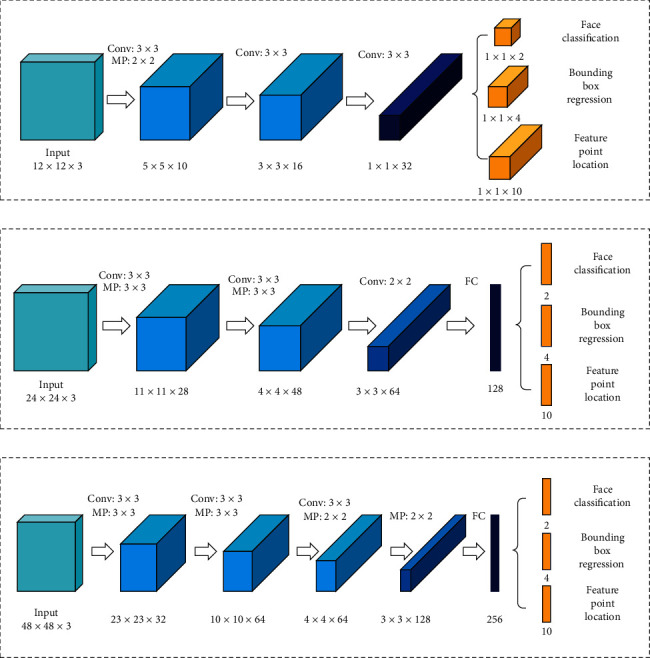
\includegraphics{img/CIN2020-7251280.002.jpg}
    \caption{L'architecture MTCNN : (a) P-Net, (b) R-Net, and (c) O-Net.}
    \label{fig:enter-label}
\end{figure}
\begin{enumerate}
    \item \textbf{}\\
    \item \textbf{}\\
    \item \textbf{}\\
\end{enumerate}
